\subsection{Experimento 3}

Como objetivo del experimento 3, se planteó realizar la medición de la resistencia de un sistema de puesta a tierra, mediante el método visto en el experimento anterior. 

\subsubsection{Medición en el laboratorio}

Para este ensayo, se empleará un Telurímetro, presentado en la sección de \textit{\nameref{sec:MTmrspt}}, del Marco Teórico; de la marca UNI-T, modelo UT522. Este es un telurímetro de 3 puntas, donde una corresponde al electrodo de corriente, otra al de tensión y la tercera punta se conecta a la toma a tierra. En esta última punta están conectadas internamente la otra terminal del multímetro y amperímetro correspondientes a los demás electrodos (se sigue teniendo 4 puntos como en la sección anterior, pero solo se ven 3 porque dos están conectados internamente). 

El ensayo se realizó el día 4 de abril del año 2024, en el laboratorio central de electrónica de la Universidad Tecnológica Nacional, Facultad Regional Córdoba. Para este, se implementó el siguiente circuito (figura \ref{fig:circtel}), con el telurímetro antes presentado.

\begin{figure}[h!]
        \centering        
        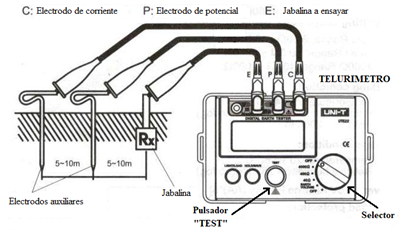
\includegraphics[width=0.8\textwidth]{Imagenes/Telurimetro.png}
        \caption{Esquema de conexión del Telurímetro UT522}
        \label{fig:circtel}
\end{figure}

Como se explico en el Marco Teórico y se puede ver en la figura \ref{fig:circtel}, para la medición de la resistencia de un sistema de puesta a tierra específico ($R_x$) se deberían insertar en el terreno los electrodos auxiliares, pero debido a que se realizó en el laboratorio, el cual cuenta con un piso de baldosas (haciendo imposible o poco práctica la inserción de los electrodos), se utilizaron dos electrodos auxiliares consistentes en dos planchas de acero de 20cm x 20cm (figura \ref{fig:electrodos}), que se apoyaran sobre el piso cubierto con un paño (trapo de piso) humedecido con bastante agua. 

\begin{figure}[h!]
        \begin{subfigure}[b]{0.5\textwidth}
        \centering  
        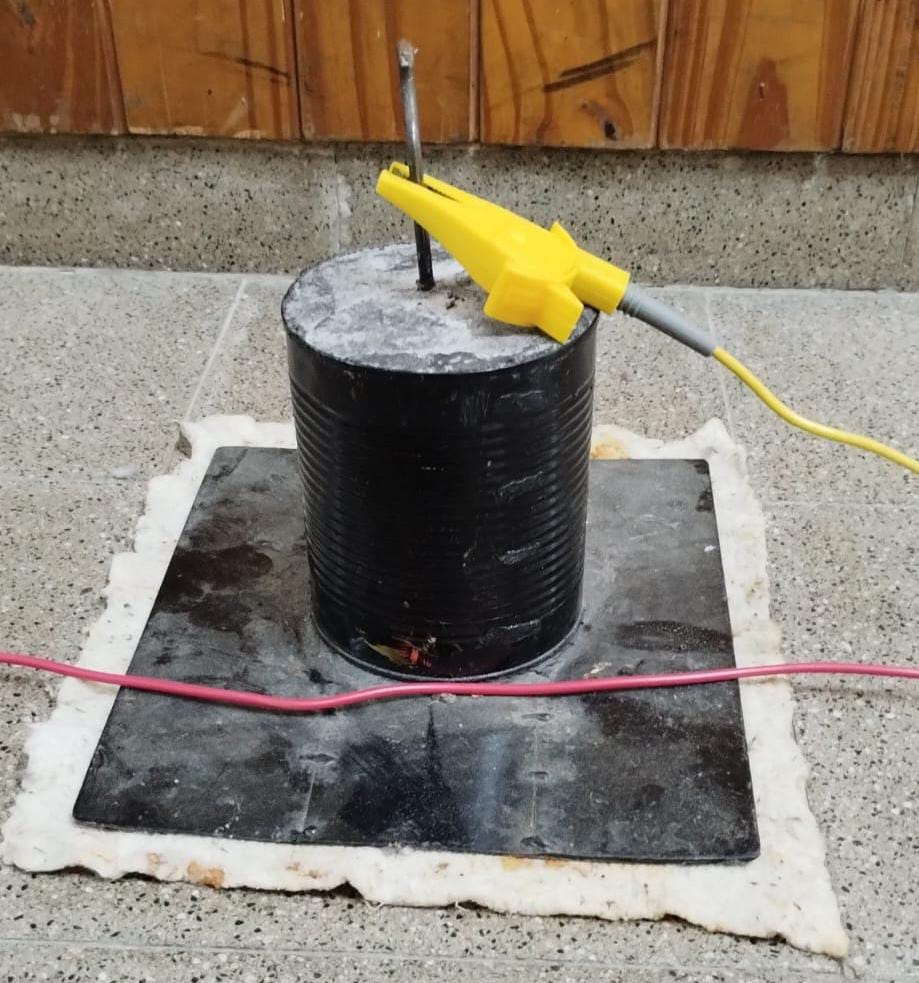
\includegraphics[width=0.6\textwidth]{Imagenes/ElectrodoTel.jpeg}
        \caption{Electrodos auxiliares utilizados}
        \label{fig:electrodos}
    \end{subfigure}
    \hfill
    \begin{subfigure}[b]{0.49\textwidth}
        \centering
        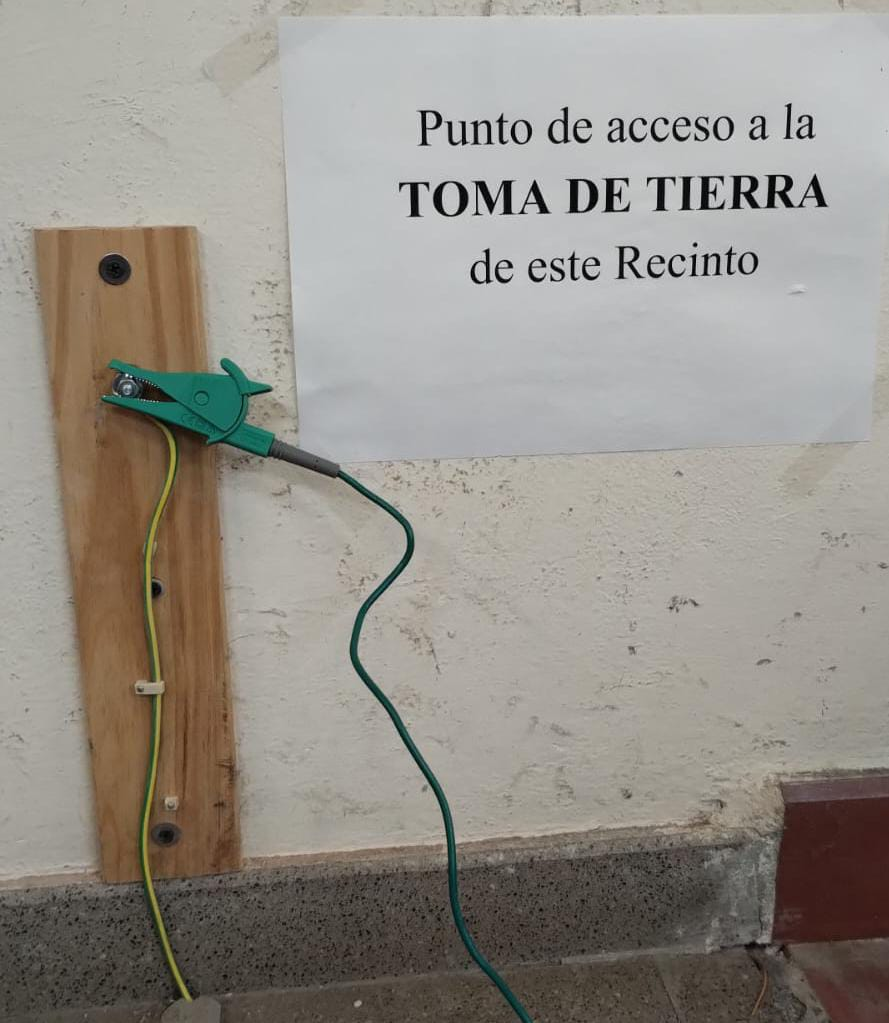
\includegraphics[width=0.57\textwidth]{Imagenes/TomaTierra.jpeg}
        \caption{Toma a tierra del laboratorio central}
        \label{fig:tomatierra}
    \end{subfigure}
    \caption{Puntos de conexión de los cables del telurímetro}
\end{figure}

Los electrodos se dispusieron en el pasillo externo, a 10 m entre sí y a aproximadamente 10 m de la toma a tierra del laboratorio central (figura \ref{fig:tomatierra}). Cabe destacar, que los electrodos fueron colocados en el pasillo, ya que en realidad la puesta a tierra del laboratorio consiste en una malla conductora colocada debajo de todo el solado del recinto. 

Una vez colocados los electrodos y conectados estos al telurímetro, se comenzó con las mediciones, comenzando desde el rango más alto del instrumento hasta llegar a la medición más precisa de acuerdo con el valor a medir. 

Siguiendo este método, el telurímetro mostró un un valor de resistencia de la jabalina de:

\begin{figure}[h!]
    \begin{minipage}{0.6\textwidth}\
        \centering  
        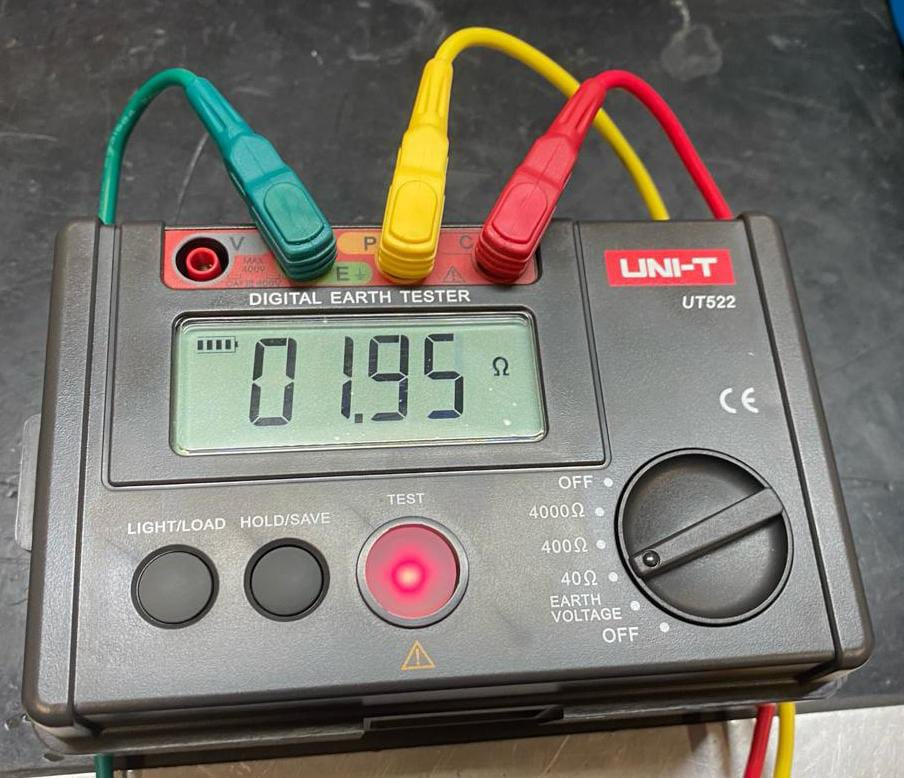
\includegraphics[width=0.6\textwidth]{Imagenes/Lecttel.jpeg}
        \caption{Lectura en el telurímetro}
        \label{fig:lecttel}
    \end{minipage}
    \begin{minipage}{0.39\textwidth}\
        \begin{equation*}
            R_{Jabalina} = 1.95 [\Omega]
        \end{equation*}
    \end{minipage}
\end{figure}

Una vez obtenido este valor, se procedió a calcular la incertidumbre de esta medición. Para esto se tuvieron en cuenta los datos de precisión del instrumento, consignados en la tabla \ref{tab:Telurimetro}, del Anexo \ref{sec:Información Instrumentos}; y la fórmula antes presentada para el cálculo de incertidumbre.

\begin{equation}
    \Delta R = \pm \left( \cfrac{2.0 \cdot 1.95 [\Omega]}{100} + 20 \cdot 10 [m\Omega] \right) = \pm 0.239 [\Omega]  
\end{equation}

Quedando como resultado de la medición el siguiente valor de resistencia:

\begin{equation*}
    R_{Jabalina} = 1.95 \pm 0.239 [\Omega]
\end{equation*}

Se puede ver que el sistema de puesta a tierra de nuestra facultad, está dentro de la norma establecida por la ley, que exige que la resistencia de este tipo de sistemas, no puede superar los 5$\Omega$. Según lo indicado por el telurímetro y suponiendo la mayor incertidumbre, el valor de resistencia no supera los 2.5$\Omega$.

Luego de realizada esta medición se reemplazó el instrumento por otro telurímetro, uno modelo MI-2124 de la marca METREL. Este segundo telurímetro era de cuatro puntos por lo que tenía cuatro entradas en lugar de tres como el anterior, y la conexión interna entre voltímetro y amperímetro no estaba. Sin embargo, esa misma conexión se realizo externamente, los cables correspondientes a un terminal del voltímetro y uno del amperímetro, se conectaron ambos a la toma a tierra del laboratorio y los dos restantes, a los electrodos.

Una vez instalado el dispositivo y los electrodos, se procedió a realizar la medición (figura \ref{fig:tel2lab}). 

\begin{figure}[h!]
        \centering        
        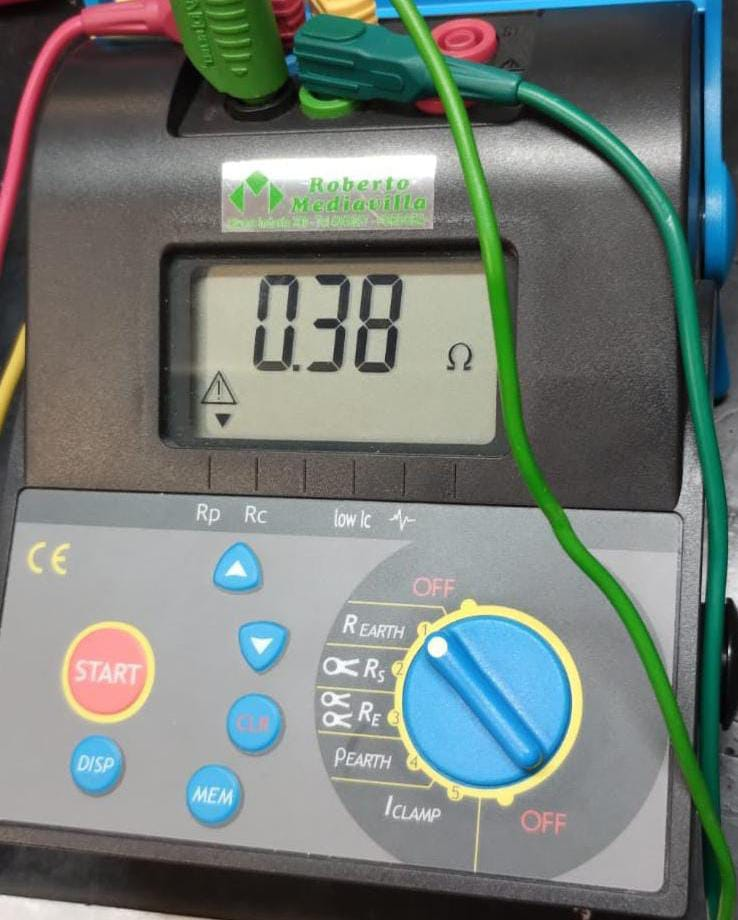
\includegraphics[width=0.3\textwidth]{Imagenes/tel2lab.jpeg}
        \caption{Medición con Telurímetro MI-2124}
        \label{fig:tel2lab}
\end{figure}

En este caso, no hizo falta el procedimiento de ir bajando de escala, ya que era de auto-rango, sin embargo se puede ver que la resistencia medida es mucho menor (0.38$\Omega$). 

En cuanto a la incertidumbre en la medición, aplicamos el cálculo anterior, con las especificaciones del nuevo telurímetro (Anexo \ref{sec:Información Instrumentos}, tabla \ref{tab:TelurMI2124}). 

\begin{equation*}
    \Delta R = \pm \left( \cfrac{2 \cdot 0.38 [\Omega]}{100} + 3 \cdot 10 [m\Omega] \right) = \pm 0.0376 [\Omega]  
\end{equation*}

Según esta segunda medicion tenemos que la resistencia del sistema de puesta a tierra es de:

\begin{equation*}
    R_{Jabalina} = 0.38 \pm 0.0376 [\Omega]
\end{equation*}

La diferencia entre las lecturas (incluyendo su incertidumbre) no debería ser tan grande, se supone que se debían obtener lecturas similares. Se cree que esta diferencia puede deberse a la utilización de electrodos distintos a los que vienen con el dispositivo y que estos agregaron cierta resistencia de contacto adicional debido a una mala conexión, que puede haberse corregido para la segunda medición. Afortunadamente, ambas mediciones indicaban que el sistema del laboratorio estaba dentro de la norma, por lo que aunque exista esta diferencia, no se debería presentar ningún problema durante su utilización.

\subsubsection{Medición en el patio frontal}

Adicionalmente, se realizó otro ensayo de la resistencia del sistema de puesta a tierra en el patio frontal de la facultad, donde esta vez si se emplearon las estacas que vienen con el dispositivo. La toma a tierra utilizada en esta ocasión se encontraba dentro de otro laboratorio que daba al patio.



Luego de colocar las estacas, se midió la resistencia de la puesta a tierra en ese punto y el telurímetro UNI-T reveló un valor más bajo que en la medición anterior (figura \ref{fig:tel1patio}). 

En este caso, el valor era de 0.27$\Omega$, que junto con la incertidumbre queda:

\begin{equation*}
    \Delta R = \pm \left( \cfrac{2.0 \cdot 0.27 [\Omega]}{100} + 20 \cdot 10 [m\Omega] \right) = \pm 0.2054 [\Omega]    
\end{equation*}

\begin{equation*}
    R_{Jabalina_1} = 0.27 \pm 0.2054 [\Omega]
\end{equation*}

En esta medición podemos ver que la exactitud de este multímetro quizá no es la más adecuada para medir una resistencia tan pequeña, ya que la incertidumbre es muy similar al valor medido. En otras palabras el error máximo que puede haber en la medición es de aproximadamente el 100$\%$ del valor. 

Manteniendo exactamente la misma disposición e incluso los mismos cables se cambió el telurímetro por el de la marca METREL, y el resultado fue el de la figura \ref{fig:tel2patio}.

\begin{figure}[h!]
        \begin{subfigure}[b]{0.5\textwidth}
        \centering  
        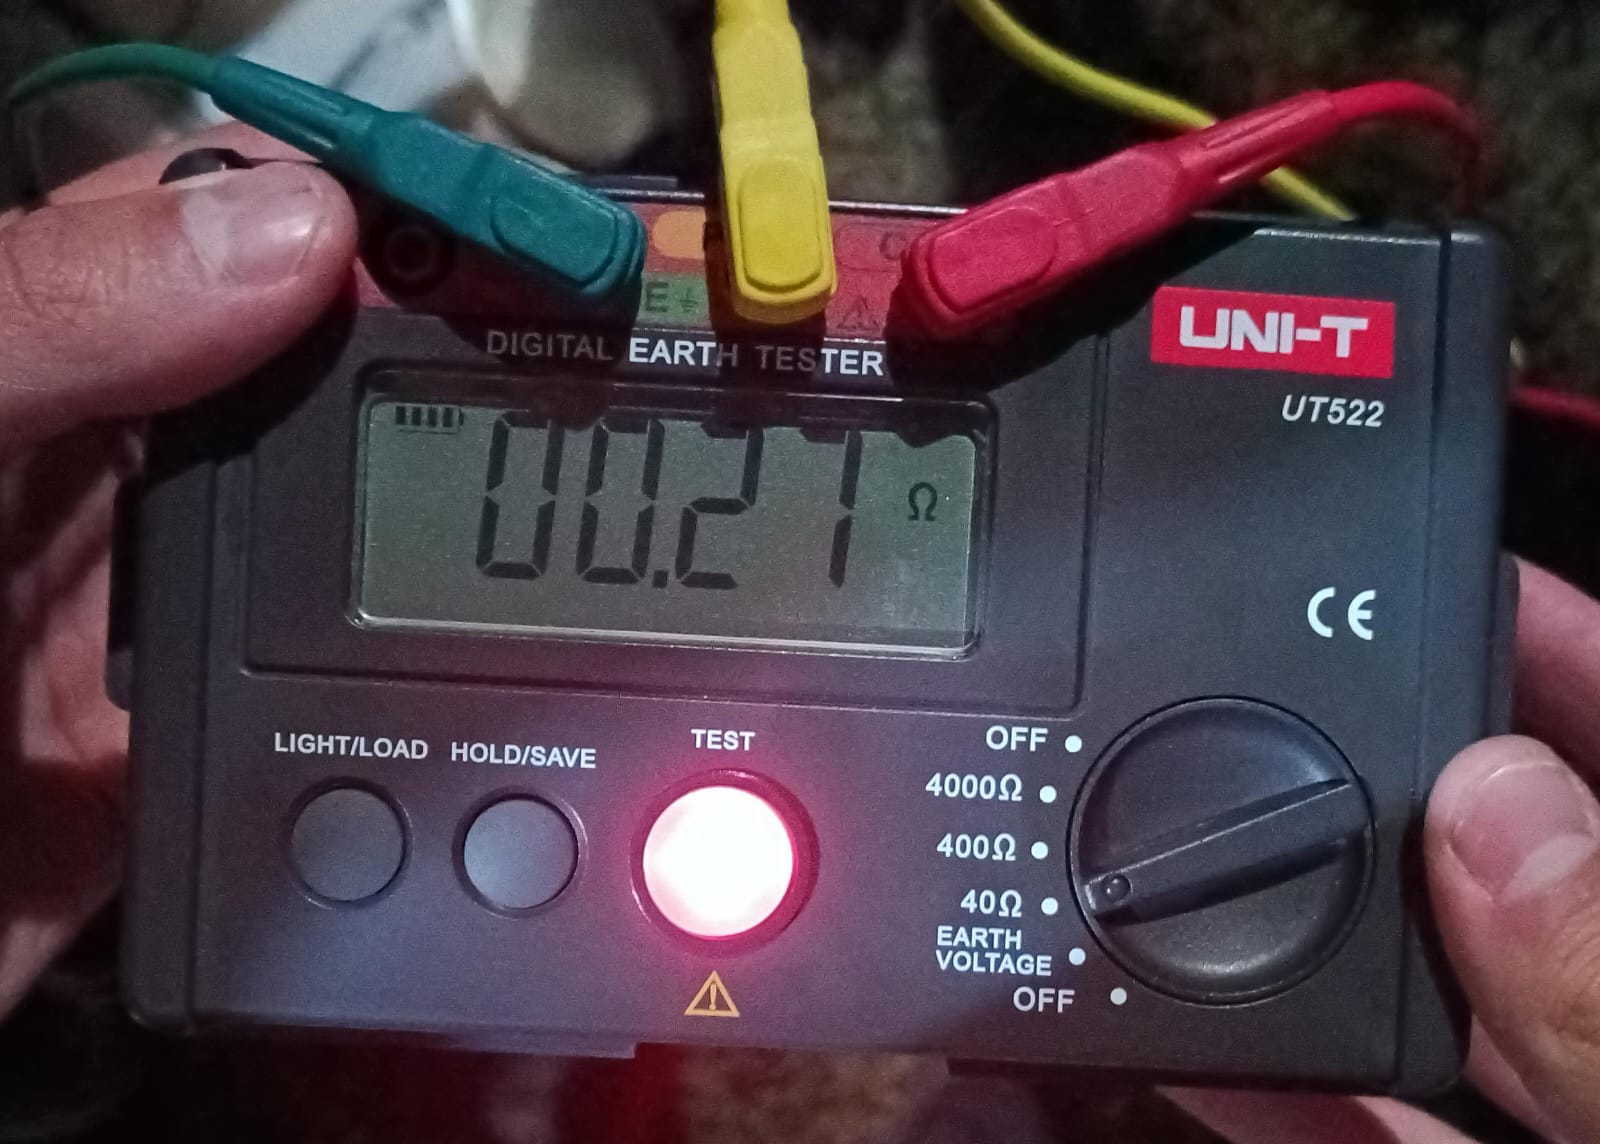
\includegraphics[width=0.8\textwidth]{Imagenes/tel1patio.jpeg}
        \caption{Medición con Telurímetro UT-522}
        \label{fig:tel1patio}
    \end{subfigure}
    \hfill
    \begin{subfigure}[b]{0.49\textwidth}
        \centering
        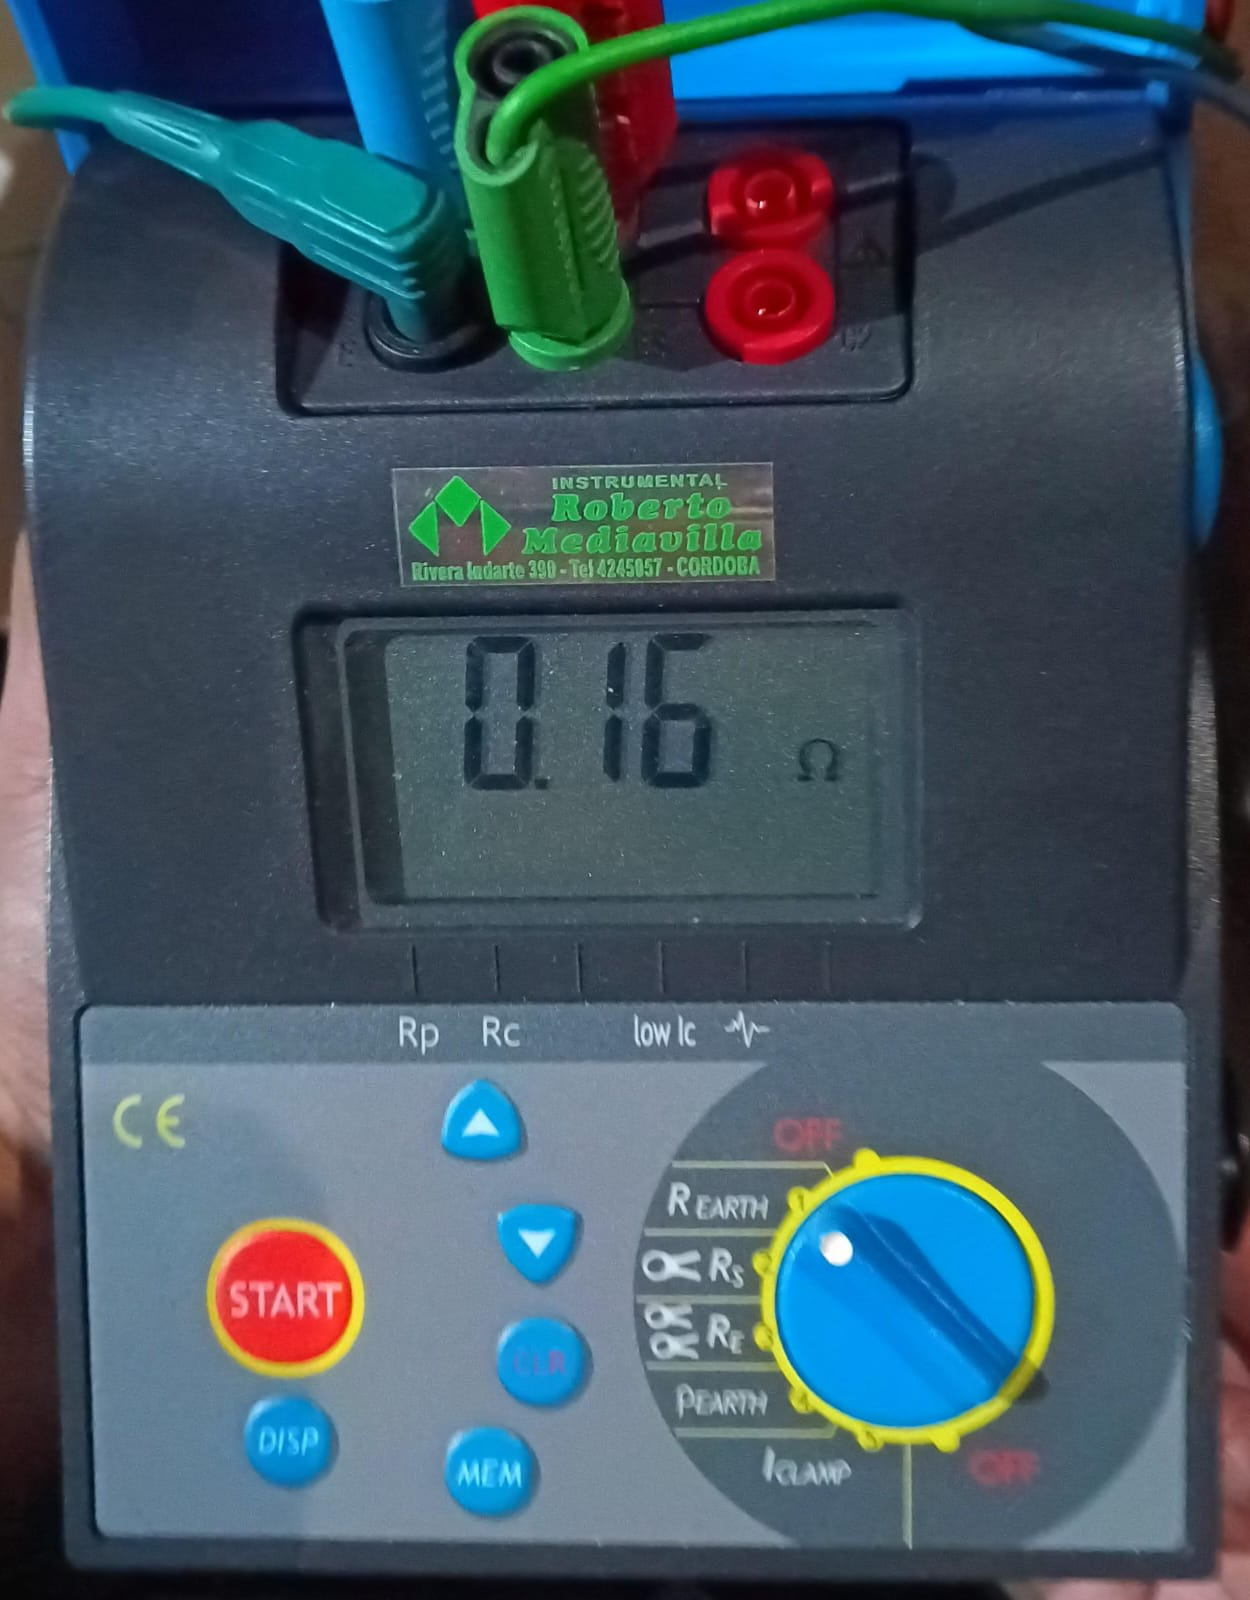
\includegraphics[width=0.45\textwidth]{Imagenes/tel2patio.jpeg}
        \caption{Medición con Telurímetro MI-2124}
        \label{fig:tel2patio}
    \end{subfigure}
    \caption{Mediciones del sistema de puesta a tierra en el patio}
\end{figure}

A simple vista se aprecia que la diferencia entre mediciones es mucho menor, pero este telurímetro sigue mostrando un valor de resistencia menor que el de marca UNI-T.

Calculamos la incertidumbre de este última medición y obtenemos:

\begin{equation*}
    \Delta R = \pm \left( \cfrac{2 \cdot 0.16 [\Omega]}{100} + 3 \cdot 10 [m\Omega] \right) = \pm 0.0332 [\Omega]  
\end{equation*}

\begin{equation*}
    R_{Jabalina_2} = 0.16 \pm 0.0332 [\Omega]
\end{equation*}

En este caso, vemos que este telurímetro es mucho más adecuado que el anterior para la medición de resistencias tan pequeñas, ya que el margen de error es muchísimo menor. Así que, en caso de tener que elegir un valor como el valor real, sería más acertado elegir este segundo valor.

%Por último y como extra para concluir con esta experiencia, se midió la resistividad de la tierra ($\rho_{tierra}$ o $\rho_{earth}$). Para este ensayo, se mantuvieron las condiciones del ensayo anterior y la medición arrojó el siguiente valor (figura \ref{fig:}): 